# 7.10 Телеоперация вашего робота


Всегда полезно поддерживать какое-то ручное управление вашим роботом, особенно при тестировании нового кода. Мы видели, что базовый контроллер для робота подписывается на тему / cmd\_vel и отображает любые опубликованные там сообщения Twist в сигналы двигателей. Если мы можем использовать устройство дистанционного управления, такое как джойстик или игровой контроллер, для публикации сообщений Twist по теме / cmd\_vel, мы можем использовать его для телеуправления роботом. (Это еще один хороший пример того, как ROS позволяет нам абстрагироваться от базового оборудования.)

К счастью, пакет \href{http://wiki.ros.org/turtlebot_teleop}{turtlebot\_teleop} уже содержит узлы для отправки команд Twist через клавиатуру, джойстик или контроллер PS3. Чтобы получить требуемые пакеты ROS, выполните команду:

```text
$ sudo apt-get install ros-indigo-joystick-drivers \ ros-indigo-turtlebot-teleop
```

Перед телеоперацией реального робота, попробуйте его с помощью симулятора ArbotiX. Поднимите поддельный TurtleBot, если он еще не запущен:

```text
$ roslaunch rbx1_bringup fake_turtlebot.launch
```

И это RViz еще не работает, запустите его сейчас:

```text
$ rosrun rviz rviz -d `rospack find rbx1_nav`/sim.rviz
```

Теперь давайте взглянем на дистанционное управление имитируемого робота с помощью клавиатуры или джойстика.

#### _7.10.1 Использование клавиатуры_

Пакет turtlebot\_teleop включает файл keyboard\_teleop.launch, который был скопирован в каталог rbx1\_nav / launch, чтобы мы могли редактировать пару параметров, описанных ниже. Используйте следующую команду для запуска этой копии файла запуска:

```text
$ roslaunch rbx1_nav keyboard_teleop.launch
```

Затем вы должны увидеть следующие инструкции на экране вашего терминала:

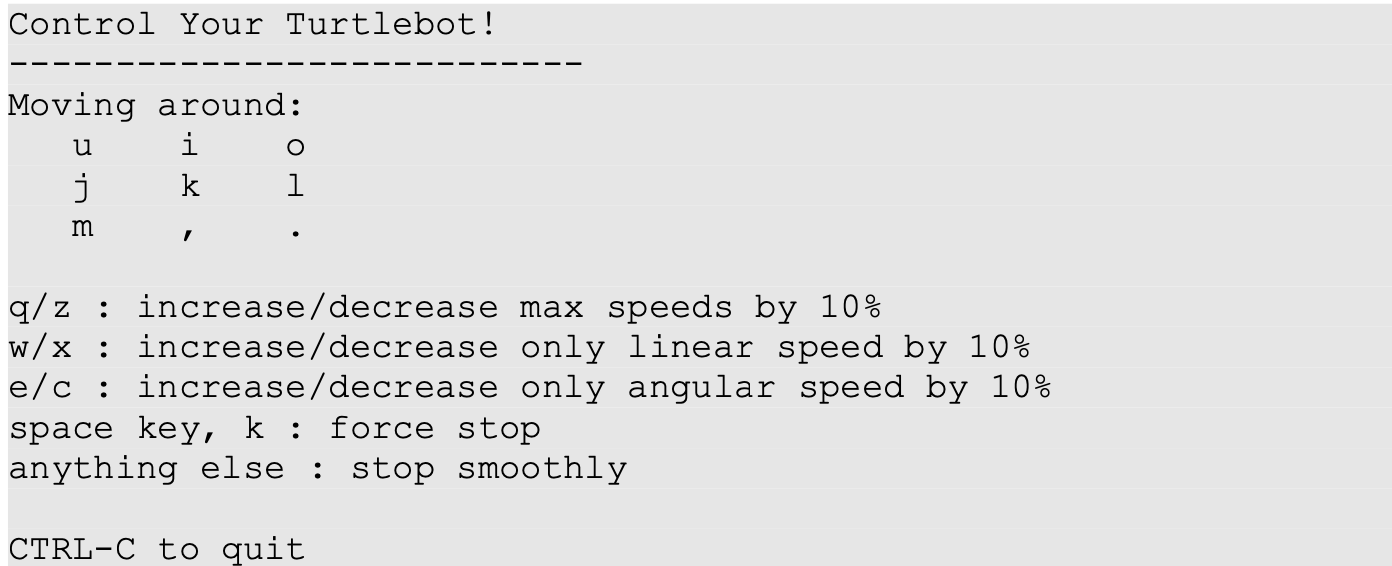
\includegraphics[width=9cm]{.gitbook/assets/snimok-ekrana-2020-05-30-v-15.20.32.png}

Наведите курсор на окно терминала Teleop, попробуйте нажать букву i. Вы должны увидеть, как фальшивый TurtleBot продвигается вперед в RViz. Обратите внимание, что если вы прекратите нажимать, робот замедлится и остановится. Попробуйте некоторые другие ключи, чтобы убедиться, что все работает.

Если вы посмотрите на файл keyboard\_teleop.launch в каталоге rbx1\_nav / launch, то увидите, что узел teleop клавиатуры принимает два параметра: scale\_linear и scale\_angular для определения линейной и угловой скорости робота по умолчанию. При первом тестировании телеоперации на реальном роботе рекомендуется установить эти значения меньше значений по умолчанию, чтобы робот двигался медленно. К сожалению, на момент написания этой статьи в пакете turtlebot\_teleop была ошибка, препятствующая чтению двух параметров узлом keyboard\_teleop, поэтому в настоящее время эти параметры будут игнорироваться.

#### _7.10.2 Использование игровой площадки Logitech_

Если у вас есть джойстик или игровая панель, вы можете использовать файл joystick\_teleop.launch в пакете turtlebot\_teleop. Мы сделали локальную копию этого файла в каталоге rbx1\_nav / launch, чтобы различные параметры можно было редактировать в соответствии с вашими потребностями. Следующее описание относится конкретно к беспроводной игровой площадке Logitech.

Для использования телеопа джойстика выполните следующую команду:

```text
$ roslaunch rbx1_nav joystick_teleop.launch
```

Если вы получили ошибку, такую ​​как:

> \[ERROR\] \[1332893303.227744871\]: Couldn't open joystick /dev/input/js0. Will retry every second.

тогда ваш джойстик или игровая панель либо не подключены к USB-порту, либо не распознаются Ubuntu. Если вы не получили никаких ошибок, нажмите кнопку «Мертвец» (см. Примечание ниже) и попробуйте переместить джойстик или левую ручку на игровой клавиатуре.

\textbf{ПРИМЕЧАНИЕ.} Если вы используете игровую панель Logitech, вы должны сначала нажать и удерживать кнопку правого указательного пальца, прежде чем робот отреагирует на левую ручку переключателя. Эта кнопка называется переключателем «мертвец», поскольку робот перестанет двигаться, если вы отпустите ее.

Вы можете отредактировать файл joystick\_teleop.launch, чтобы изменить масштабные коэффициенты для линейной и угловой скорости. Вы также можете отобразить переключатель мертвецов на другую кнопку. Чтобы узнать номера, соответствующие каждой кнопке, попробуйте программу jstest:

```text
$ sudo apt-get install joystick
$ jstest /dev/input/js0
```

Затем нажмите различные кнопки и посмотрите на цифры в нижней части экрана, чтобы увидеть, какая из них переключается с «выключено» на «включено». Введите Ctrl-C, чтобы закрыть тестовый экран.

#### _7.10.3 Использование графического интерфейса контроллера ArbotiX_

Вы можете настроить интерфейс с помощью следующей команды:

```text
$ arbotix_gui
```

Чтобы переместить вашего робота, нажмите и удерживайте красную точку с помощью мыши . Затем переместите, переместите точку в направление, в котором вы хотите, чтобы ваш робот двигался. Старайтесь не перемещать его слишком далеко, так как скорость робота зависит от расстояния от источника. Если вы используете симулятор Pi Robot, вы также увидите элементы управления для суставов рук, как показано ниже:

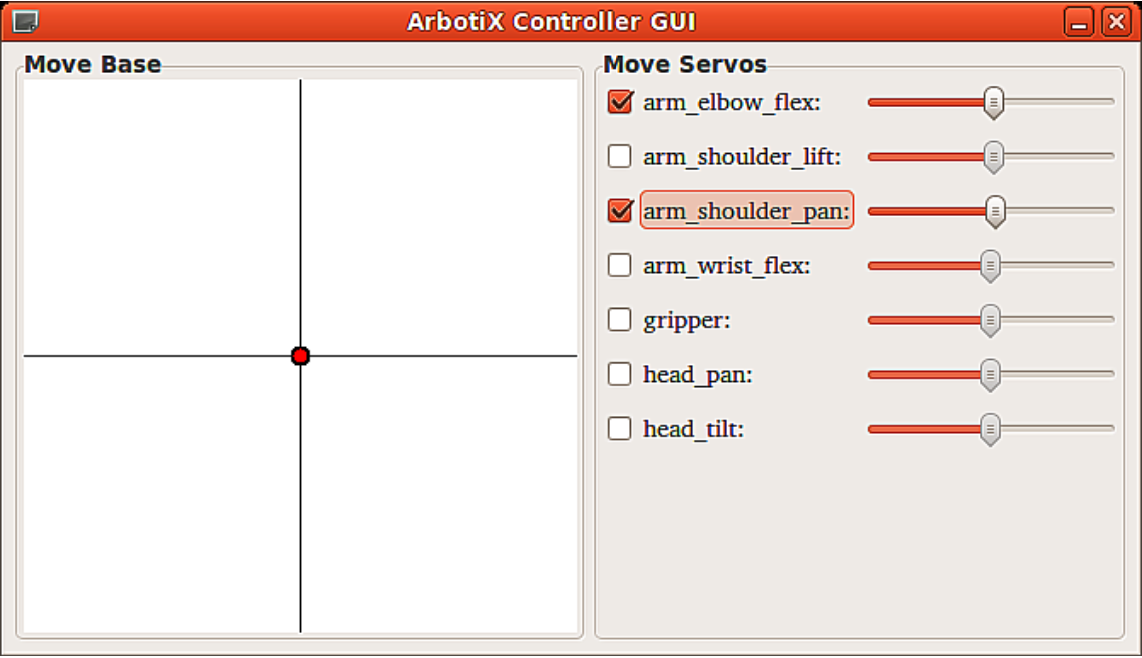
\includegraphics[width=9cm]{.gitbook/assets/snimok-ekrana-2020-05-30-v-15.30.55.png}

Чтобы переместить одно из соединений в симуляторе, установите флажок рядом с именем сервопривода, затем используйте ползунок.

7.10.4 Телеоперация TurtleBot с использованием интерактивных маркеров

Метапакет Turtlebot включает в себя очень интересный пакет интерактивных маркеров, который позволяет перемещать настоящего робота, перетаскивая элементы управления в RViz. Инструкции по его использованию представлены на вики-странице \href{http://ros.org/wiki/turtlebot_interactive_markers/Tutorials/UsingTurtlebotInteractiveMarkers}{turtlebot\_interactive\_markers}, хотя эта страница не обновлялась с Groovy. (Нажмите на вкладку Groovy в верхней части страницы, как только она появится.)

Чтобы установить пакет для ROS Indigo, выполните команду:

```text
$ sudo apt-get install ros-indigo-turtlebot-interactive-markers
```

Чтобы попробовать это с поддельным TurtleBot, выполните следующие команды:

```text
$ roslaunch rbx1_bringup fake_turtlebot.launch
```

Откройте RViz с помощью предварительно сконфигурированного файла конфигурации interactive\_markers.rviz:

```text
$ rosrun rviz rviz -d `rospack find rbx1_nav`/interactive_markers.rviz
```

Наконец, откройте файл interactive\_markers.launch в пакете rbx1\_nav:

```text
$ roslaunch rbx1_nav interactive_markers.launch
```

Этот файл запуска был скопирован из пакета turtlebot\_interactive\_markers и немного изменен для работы с поддельным TurtleBot.

Вернувшись в RViz, нажмите кнопку Взаимодействовать вдоль верхней панели инструментов. Экран RViz должен выглядеть следующим образом:

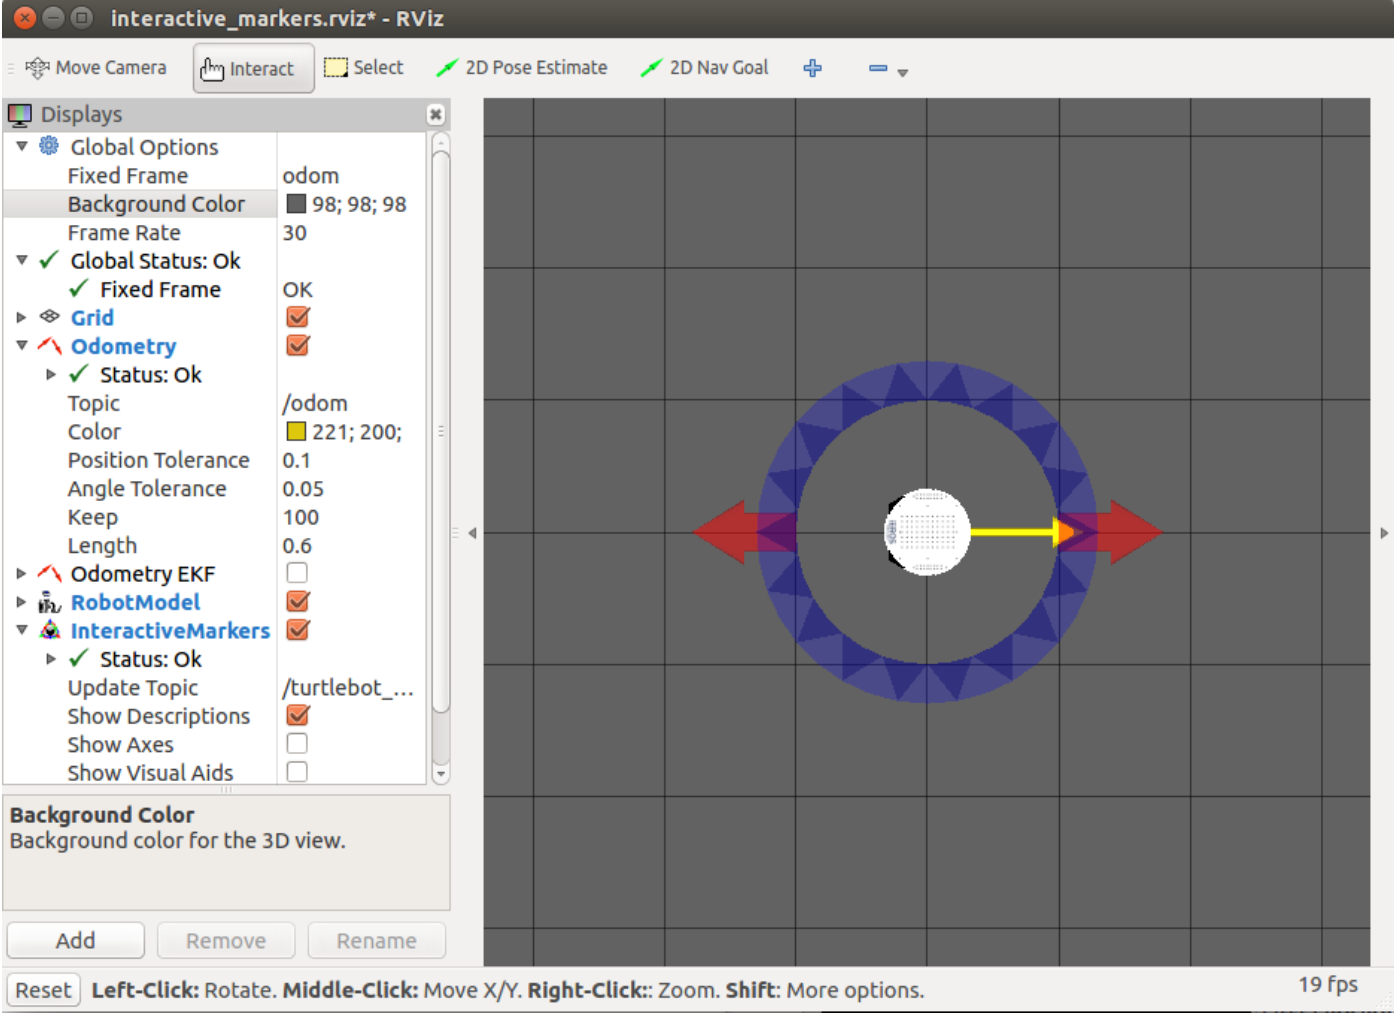
\includegraphics[width=9cm]{.gitbook/assets/snimok-ekrana-2020-05-30-v-15.33.16.png}

Нажмите на красные стрелки, чтобы переместить поддельного робота вперед или назад и поверните синее кольцо, чтобы повернуть робота.

